%        File: pwe2.tex
%     Created: Thu Apr 25 10:00  2019 S
% Last Change: Thu Apr 25 10:00  2019 S
%
\documentclass[a4paper, 12pt]{article}

\usepackage[T1]{fontenc}
\usepackage[]{amsmath, amssymb}
\usepackage{IEEEtrantools}
\usepackage[]{graphicx}
\usepackage{booktabs}
\usepackage{float}
\usepackage[toc, page]{appendix}
\usepackage[]{hyperref}

\title{Power Electronics: Designing and Building a Single Switch Flyback Converter}
\author{Ruan de Bruyn \and 216054484 \and Quintin Kruger \and 216008466}

\begin{document}

\pagenumbering{gobble}
\maketitle
\newpage
\pagenumbering{roman}
\tableofcontents
\listoffigures
\newpage
\pagenumbering{arabic}

\section{Introduction}

The purpose of this practical was to design and construct a Flyback converter.
The design specifications of this converter are given to us in the practical
guide, and this report shows the steps and reasoning we had while building the
converter. It's also worth noting that the practical guide recommended a
textbook on designing switching power supplies \cite{pressman}, which was used
extensively to understand and design a practical real-life flyback converter.

% endsection Introduction

\section{Literature Review}

A Flyback Converter is a very versatile DC-DC converter design for low power
applications, and can essentially be derived from a buck boost converter,
except for the important distinction that a coupled inductor is used instead.
The reason for this is because it provides isolation between the primary and
secondary circuits, and according to \cite{pressman}, it is ``particularly
valuable in low-cost multiple output power supplies yielding a significant
saving in cost and space''. A typical flyback topology is shown in Figure
\ref{fig:pressman_circuit}.

\begin{figure}[H]
  \centering
  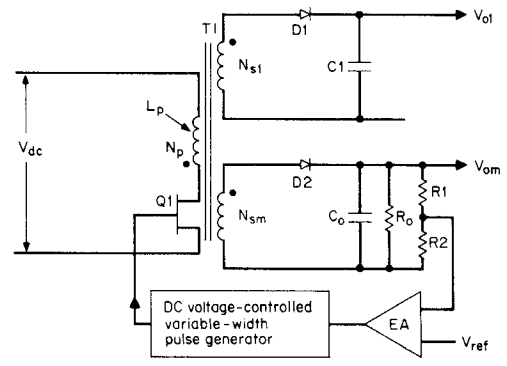
\includegraphics[width=.6\textwidth]{./images/pressman_circuit.png}
  \caption{Master/slave flyback converter with negative feedback loop \textit{(\cite{pressman} Figure 4.1 (a))}}
  \label{fig:pressman_circuit}
\end{figure}

A comprehensive analysis of this circuit topology can be found in
\cite{pwe_conv_applications}, where the key waveforms for a flyback converter
topology can be seen below in Figure

\begin{figure}[H]
	\centering
	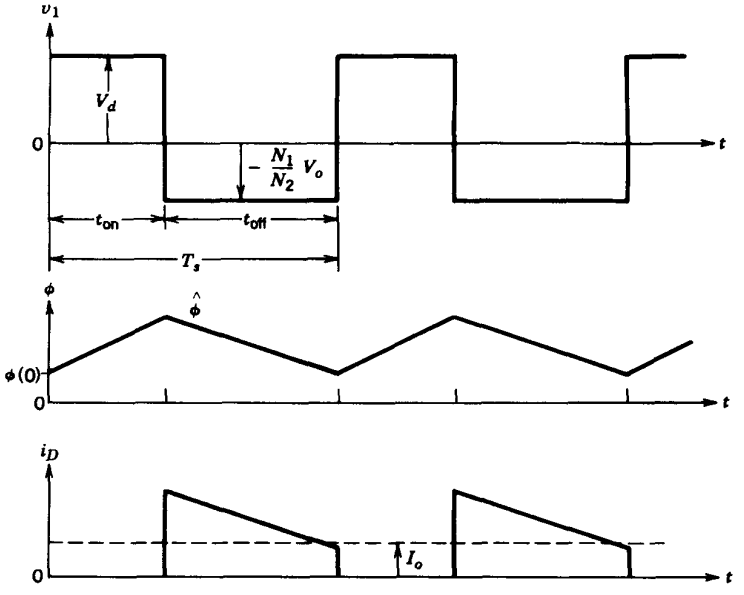
\includegraphics[width=.8\textwidth]{./images/pwe_text_flyback_waveforms.png}
	\caption{Flyback Topology Waveforms \textit{(\cite{pwe_conv_applications}, Figure 10-8)}}
	\label{fig:pwe_text_waveforms}
\end{figure}

where $v_1$ is the voltage over the primary side transformer, $\phi$ is the
flux in the coupled inductor core, and $i_D$ is the current flowing through the
secondary side diode. The derivation that relates the transfer function to the
duty cycle can be derived by taking into account the fact that the core flux
$\phi$ is constant; that is, at the start of every duty cycle $D, \{D: 0 \le D <
1\}$, $\phi(0)$ is the same value. We omit the full derivation, which can be
seen in \cite{pwe_conv_applications}, and give the full transfer function
equation as

\begin{equation}
	\frac{V_o}{V_i} = \frac{N_2}{N_1}\frac{D}{1 - D}
	\label{eq:lit_review_tf}
\end{equation}

\cite{pressman} addresses the next important design consideration ---
continuous operation mode vs discontinuous operation mode. The discontinuous
operating mode has ``dead time'', which essentially means that there is a
portion of the duty cycle where the current in the primary and secondary of the
inductor is zero, essentially ensuring that the flux stays constant because
$\phi(0) = 0$ at the start of every cycle. The continuous operation mode
doesn't have this feature, and has $\phi(0) \not = 0$ at the start of every
cycle.

Discontinuous mode flyback converters have several disadvantages according to
\cite{pressman}, including that ``secondary peak current \dots can be between
two and three times larger than that in the continuous mode''. With this comes
larger transients in output voltage, and requires large output capacitances to
counter ripple voltage. Despite this, the discontinuous mode is used more often
due to its rapid dynamic response and smaller footprint on circuits.

The continuous mode is more difficult to control in a negative feedback loop,
and if used can lead to core saturation and undesirable performance of the
converter, but is very desirable for low power circuit due to small secondary
side rms current.

% endsection Literature Review

\section{Design}

\subsection{Circuit Design}

This section discusses the design of the flyback converter. Our design follows
a single switch topology, and is shown below in figure
\ref{fig:circuit_diagram}. Note that $V_2$ is our control block, and denotes
the PWM output driving the MOSFET. There is also a negative control loop
returning from $R_2$ for measuring load voltage, as will be discussed in later
sections. A more formal diagram of the flyback circuit we based our overall
design on can be seen in figure \ref{fig:pressman_circuit}.

\begin{figure}[H]
  \centering
  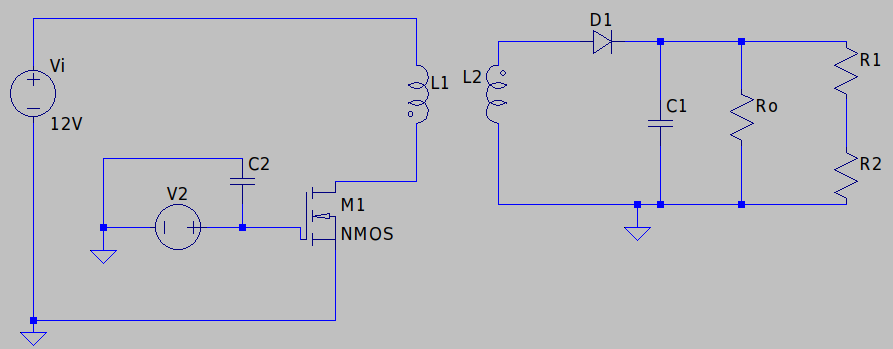
\includegraphics[width=\textwidth]{./images/circuit_diagram.png}
  \caption{Flyback Converter Circuit}
  \label{fig:circuit_diagram}
\end{figure}

\noindent 

\subsubsection{Design Specifications}

The student number we used to get the design specifications was 216054484.
Following the practical guide, our design specifications are given as such:

\begin{table}[H]
  \centering
  \begin{tabular}{r c c}
    \toprule
    \textbf{Attribute} & \textbf{Symbol} & \textbf{Value} \\
    \midrule
    Power & $P_o$ & 20W \\
    Efficiency & $\eta$ & 80\% \\
    Maximum duty cycle & $D_{\text{max}}$ & 42.5\% \\
    Output voltage & $V_o$ & 18V \\
    Voltage ripple & $\Delta V_o$ & 10\% \\
    Switching frequency & $f_{\text{sw}}$ & 25 kHz \\
    \bottomrule
  \end{tabular}
  \caption{Design Specifications}
  \label{tab:design_specs}
\end{table}

\subsubsection{Load Resistance}

Since we have output power and output voltage specified, we start with
calculating the load resistance:

\begin{IEEEeqnarray}{rCl}
  P_o & = & \frac{V_o^2}{R_o} \nonumber \\
  R_o & = & \frac{V_o^2}{P_o} \nonumber \\
  & = & \frac{18^2}{20} \nonumber \\
  & = & 16.2\Omega
  \label{eq:load_resistor}
\end{IEEEeqnarray}

\subsubsection{Turns ratio}

We used the recommended textbook the practical suggested \cite{pressman} during the
design of this converter. Since we have a switching frequency of $f_s = 25kHz$,
that leaves us with a period of

\begin{IEEEeqnarray}{rCl}
	T & = & \frac{1}{f_s} \nonumber \\
	& = & 40 \mu s
	\label{eq:T}
\end{IEEEeqnarray}

For stability and dynamic response reasons, we decided to have this flyback
converter operate in discontinuous mode. Thus, we will have an ``on'' time,
$T_{on}$, which will represent our duty cycle. There needs to be a ``reset''
time as well, to allow the inductor to completely dispose of the energy in its
magnetic field. \cite{pressman} recommends the following constraint:

\begin{equation}
	T_{on} + T_r = 0.8T
	\label{eq:time_constraint}
\end{equation}

Equation \eqref{eq:time_constraint} ensures that there is enough dead time
between cycles for the inductor to reset. Then, with our maximum duty cycle
being 42.5\%, we have

\begin{equation}
	T_{on} = D_{\text{max}} T = 17 \mu s
	\label{eq:ton}
\end{equation}

\noindent and from equation \eqref{eq:time_constraint}

\begin{IEEEeqnarray}{rCl}
	T_r & = & 0.8(40 \mu s) - 17 \mu s \nonumber \\
	& = & 15 \mu s
	\label{eq:tr}
\end{IEEEeqnarray}

leaving us with a dead time of about $8 \mu s$ per cycle to ensure
discontinuous mode operation. Next, we need to calculate the turns ratio for
the coupled inductor. With the assumed efficiency of $\eta = 80\%$ and a
specified output power of $P_o = 20 W$, this means we would have input power
$P_i = 25 W$. From a 12V DC power supply, we would then expect to draw an
average current of approximately 2A on the primary side. This is important,
because when calculating our turns ratio, the voltage drop across the switch on
the primary side needs to be taken into account. According to the IRF510 Power
MOSFET datasheet, it has an $R_{DS, on}$ of $0.54\Omega$. Granted, this was
measured with a primary current of 3.4A according to the datasheet, but this
should suffice as an approximation for us. Then we have a forward voltage drop
over the switch of approximately $V_{DS} = (2)(0.54) \approx 1V$. 

Then, on the secondary side, we require an output voltage of $V_o = 18V$.
However, our fast switching 1N4148 diode has a forward voltage drop of $V_f =
1V$, which means that the coupled inductor has to step up voltage to compensate
for this drop. Taking all of this into account, together with the fact that the
integral of the volt-seconds over the inductor should equal zero, we have

\begin{equation}
	(V_i - V_{DS})T_{on} = \frac{N_p}{N_s}(V_o + V_f)T_r
	\label{eq:turnsratio}
\end{equation}

Letting $\rho$ denote our turns ratio, and substituting for our known values,
it follows from \eqref{eq:turnsratio} that

\begin{IEEEeqnarray}{rCl}
  \rho & = & \frac{(V_i - V_{DS})T_{on}}{(V_o + V_f)T_r} \nonumber \\
	& = & \frac{(12 - 1)17 \times 10^{-6}}{(18 + 1)15 \times 10^{-6}} \nonumber \\
	& = & 0.656 \nonumber \\
	& \approx & 0.65
	\label{eq:rho}
\end{IEEEeqnarray}

\subsubsection{Primary and Secondary Side Inductances}

The inductance of the primary side of the coupled inductor comes next. The
proof of the equation for the primary inductance is covered in Pressman
\cite{pressman}, and is beyond the scope of this report. We will, however,
alter the equation as a function of efficiency (\cite{pressman} assumes a fixed
efficiency), which yields

\begin{equation}
	V_o = V_{i} T_{on} \sqrt{\frac{R_o}{\tfrac{2}{\eta}T L_p}} \Rightarrow L_p = \frac{(V_i T_{on})^2}{\tfrac{2}{\eta} T P_o}
	\label{eq:lp}
\end{equation}

Substituting our values, it leaves us with a primary inductance of

\begin{IEEEeqnarray}{rCl}
	L_p & = & \frac{(12 \times 17 \times 10^{-6})^2}{\tfrac{2}{0.8}(40 \times 10^{-6})(20)} \nonumber \\
	& = & 2.08 \times 10^{-5} \nonumber \\
	& = & 20.8 \mu H
	\label{eq:primary_inductance}
\end{IEEEeqnarray}

Getting the secondary inductance can be done with a simple ratio:

\begin{IEEEeqnarray}{rCl}
	L_s & = & \rho^{-2}L_p \nonumber \\
	& = & 0.65^{-2}(2.08 \times 10^{-5}) \nonumber \\
	& = & 4.925 \times 10^{-5} \nonumber \\
	& = & 49.3 \mu H
	\label{eq:secondary_inductance}
\end{IEEEeqnarray}

\subsection{Inductor Design} % (fold)
\label{sub:inductor_design}
Now that we have the required inductance we can determine the number of turns
we need on the primary side and the secondary side respectively using a core
that has an air-gap total length of $\sum g = 3\times 10^{-3}m$ and an air gap
total area of $A_g = 2.4\times10^{-5}m^2$. From Mohan
\cite{pwe_conv_applications}, using these specifications we calculated the
number of windings onto an E42 gapped core using the equation that follows

\begin{equation}
	\label{eq:windings}
	L = \frac{N^2A_g\mu}{\sum g}
\end{equation}

where $L$ is the inductance for which we are designing, $N$ the number of
windings and $\mu$ the permeability of air which is $4\pi\times 10^{-7}$.
Equation \eqref{eq:windings} was arrived at using a derivation which is again
beyond the scope of this report but can be seen from
\cite{pwe_conv_applications}. \\

For primary-side inductance, the primary-side turns needed are calculated below
\begin{equation}
	\begin{array}{rll}
		20.8\times 10^{-6} &= &1.005\times 10^{-8}N_p^2\\
		N_p & = & 46\\ 
	\end{array}
\end{equation}

Now from the turns ratio calculated to be $0.65$, the turns needed on the
secondary side yielding this ratio is $N_s = 71$ 

\subsubsection{Peak Currents and Capacitance}
In order to double check our peak currents, we can use the current through an
inductor equation, where

\begin{equation}
  i_L = \frac{1}{L} \int V_L dt
  \label{eq:inductor_current}
\end{equation}

\noindent Denoting peak primary current as $\hat{I_p}$, we get our primary peak current as
\begin{IEEEeqnarray}{rCl}
  \hat{I_p} & = & \frac{1}{L_p} \int_0^{T_{on}} V_i dt \nonumber \\
  & = & \frac{12}{20.8 \times 10 ^{-6}}(17 \times 10^{-6}) \nonumber \\
  & = & 9.8 A
  \label{eq:primary_current_peak}
\end{IEEEeqnarray}

\noindent In order to get the peak secondary current, we simply multiply it with $\rho$,
and get

\begin{IEEEeqnarray}{rCl}
  \hat{I_s} & = & \hat{I_p}\rho \nonumber \\
  & = & (9.8)(0.65) \nonumber \\
  & = & 6.38 A
\end{IEEEeqnarray}

Following a derivation in Chapter 2 of Pressman \cite{pressman}, we can get the
RMS current on both sides using the formula

\begin{equation}
  I_{rms} = \frac{\hat{I}}{\sqrt{3}}\sqrt{\frac{T'}{T}}
  \label{eq:rms_current_equation}
\end{equation}

Applying this formula with the results obtained for peak currents, we have

\begin{IEEEeqnarray}{rCl}
  I_{rms(primary)} = 3.69A \\
  I_{rms(secondary)} = 2.25A \label{eq:is_rms}
\end{IEEEeqnarray}

We can use the secondary rms current obtained above to calculate
the value of output capacitor $C_1$ with the following equation:

\begin{IEEEeqnarray}{rCl}
  I & = & C \frac{\Delta V}{\Delta t} \nonumber \\
  C & = & \frac{\Delta t}{\Delta V} I
  \label{eq:co_formula}
\end{IEEEeqnarray}

Taking into account the fact that the capacitor must discharge current through
an entire period except $T_r$, and that output ripple should at most be 10\% of
our output voltage, equation \eqref{eq:co_formula} gives us

\begin{IEEEeqnarray}{rCl}
  C_1 & = & \frac{25 \times 10^{-6}}{0.1(18)}(2.25) \nonumber \\
  & = & 3.1304 \times 10^{-5} \nonumber \\
  & = & 31.3 \mu F \label{eq:co}
\end{IEEEeqnarray}

% endsubsection Circuit Design

\subsection{Negative Feedback Control}

We decided to use a Raspberry Pi Model 3B+ as our PWM source for this circuit.
We made this choice because the Raspberry Pi has ample processing power for
this application; its 1.4GHz processor can perform elementary operations with
sub-microsecond speed, and will ensure that our duty cycle --- which is on the
order of microseconds --- will stay constant while sensor data from the circuit
is being processed.

The MCP3008 IC was used as an analog-to-digital converter. This IC outputs a
digital signal to the Raspberry Pi via the Serial SPI interface with as a ratio
of the reference voltage provided to the chip with the formula

\begin{equation}
  V_{\text{digital}} = \frac{V_{\text{analog}}}{1024} V_{\text{ref}}
  \label{eq:mcp_formula}
\end{equation}

where $V_{\text{digital}}$ is quantized to be an integer. However, the MCP3008
can only take a maximum $V_{\text{ref}}$ of 5.5V, according to the datasheet,
meaning we need to step down our load voltage to be less than that if we are to
implement effective control (and not damage the chip). This is done by the
voltage divider resistors that are parallel to the load. From Figure
\ref{fig:circuit_diagram}, these voltage dividers are denoted $R_1$ and $R_2$.
For these voltage dividers, we require that both $R_1$ and $R_2$ must be much
larger than the load, or else the branch will draw too much current and alter
the output voltage. We choose $R_1 = 100k\Omega$ and $R_2 = 10k\Omega$, and
then we have $R_1 + R_2 >> R_o$ as required.  Since the voltage over the
smaller resistor is measured by our A/D converter, we essentially step down our
load voltage as given by \eqref{eq:voltage_divider}.

\begin{equation}
  V_{\text{analog}} = \frac{10}{100 + 10}V_o = \frac{1}{11} V_o
  \label{eq:voltage_divider}
\end{equation}

Now, we supply the A/D converter with a reference voltage of $V_{\text{ref}} =
5.2V$, from the 5V DC output of the Raspberry Pi (the documentation says that
the output is 5V, but we measured it to be 5.2V). This means that our load can
have an output voltage of $11 \times 5.2 = 57.2V$ before the IC will start
giving erroneous output or become damaged. Since our output voltage is 18V, we
feel that this adds a sufficient buffer to protect the Raspberry Pi and the IC.
Also, with a reference voltage of 5.2 volts, the A/D converter has a voltage
resolution of approximately $5.2V / 1024 \approx 5mV$, which is more than
sufficient for controlling the output voltage of the converter. The actual code
for negative feedback control is given in Appendix \ref{sec:feedback_code}.

The PWM that this code ultimately controls is supplied from the Raspberry Pi to
the circuit via an ICL7667 inverting MOSFET driver, which steps up the 3.3V PWM
from the Raspberry Pi to a 12V signal. This can comfortably drive our MOSFET
past its threshold gate voltage. The MOSFET driver has protection circuitry
internally built into the package, which not only serves to protect the driver
from any inductive effects from our MOSFET, but also protects the Raspberry Pi.
When we initially built the circuit, we noticed large spikes at the output of
of the driver, and followed advice from the manufacturer's datasheet and put a
small capacitor at the output of the driver to even out the spikes somewhat.
The resultant waveforms can be seen in Figure \ref{fig:pwm_output_from_chip}.


% endsubsection Negative Feedback Control

% subsection inductor_design (end)

% endsection Design
\section{Construction}

\subsection{Components Used}

For the control block and PWM output, we used the following components:
\begin{itemize}
  \item Raspberry Pi. Used for implementing control loop and providing PWM
    output.
  \item MCP3008 A/D converter. As discussed earlier, that provides digital
    voltage readings for the control loop running via the Raspberry Pi.
  \item ICL7667 MOSFET driver. Converts 3.3V Raspberry Pi PWM to 12V PWM for
    driving MOSFET.
  \item 3.9 nF Film Capacitor. This is capacitor $C_2$ in the circuit. Reduces
    PWM switching spikes, and the type was chosen due to the reliability and
    generally long service life of film capacitors.
\end{itemize}

\noindent
The components of the converter itself are listed below
\begin{itemize}
  \item $M1$: IRF510 Power MOSFET. A reliable MOSFET we've used previously and
    are familiar with. Additionally, a robust heat sink was also added to keep
    it cool under operating conditions.
  \item $D_1$: 1N4148 diode. This diode is a fast switching type; useful for
    minimizing switching losses.
  \item $C_1$: $47 \mu F$. This capacitor is a \textit{low ESR} capacitor, and
    was chosen because this property further minimizes power losses in the
    circuit. It is larger than the result found in \eqref{eq:co}, to provide an
    extra margin for ripple current, but not excessively large such that it
    takes up a lot of space or makes the circuit significantly more costly.
  \item $R_o$: We were unable to get a load matching exactly $16.2\Omega$, as
    found in \ref{eq:load_resistor}. We used two $33\Omega$ 10W resistors for a
    load instead. When combined, they give a combined resistance of
    $16.5\Omega,\, 20$W, which is acceptable in our case.
  \item $R_1$: $100k\Omega$ resistor, rated at 0.5W
  \item $R_2$: $10k\Omega$ resistor, rated at 0.5W
\end{itemize}

\noindent
The inductor was built by adding masking tape to the outer legs of the E-core
to make up $1mm$ air gap lengths on the $3$ leg of the E-core. This yielded the
designed for air gap area and air gap total length. Windings were wound around
the  E-42 core bobbin in an interleaving manner, half of the secondary windings
were wound after which the primary windings were wound followed by the last
half of the secondary windings (with  primary windings sandwiched between the
secondary windings). The core was placed within the bobbin and masking tape was
used to keep the E-core halves and the bobbin together. 



\subsection{Final Circuit}
Figure \ref{fig:flyback_converter_build} shows the final build of the fly-back
converter and the PWM and feedback system connection of the flyback converter
to the raspberry pi.
\begin{figure}[H]
  \centering
  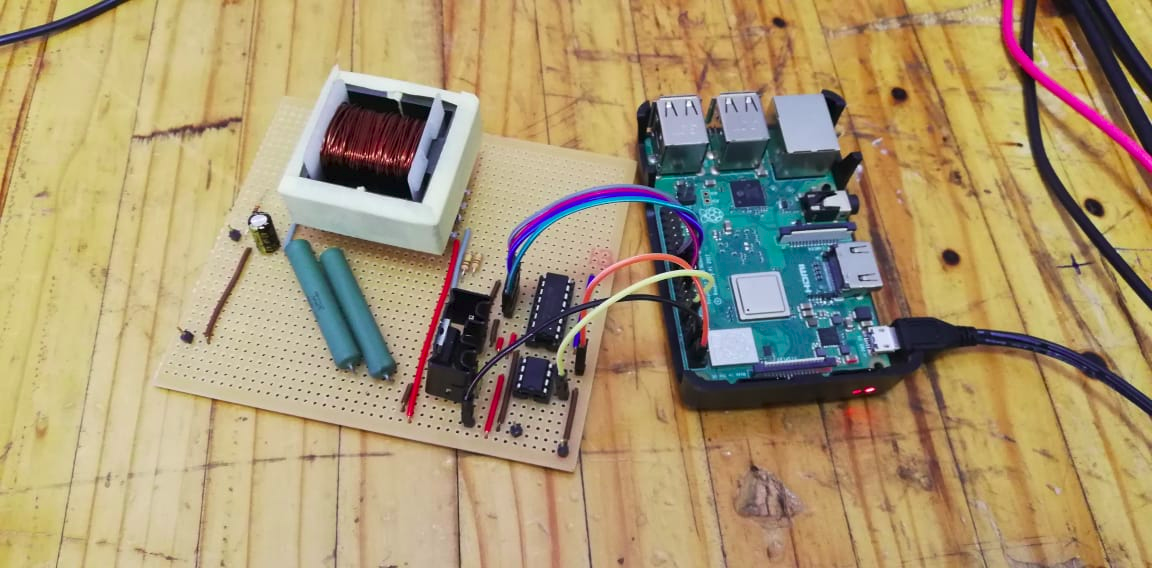
\includegraphics[width=\textwidth]{images/final_circuit_image.png}
  \caption{Final build of the Flyback converter}
  \label{fig:flyback_converter_build}
\end{figure}

% endsection Construction

\section{Results and Discussion}
The oscilloscope images of various parts of the fly-back converter are shown respectively by the figures that follow and a brief discussion of what each images tells us is given.

\begin{figure}[H]
  \centering
  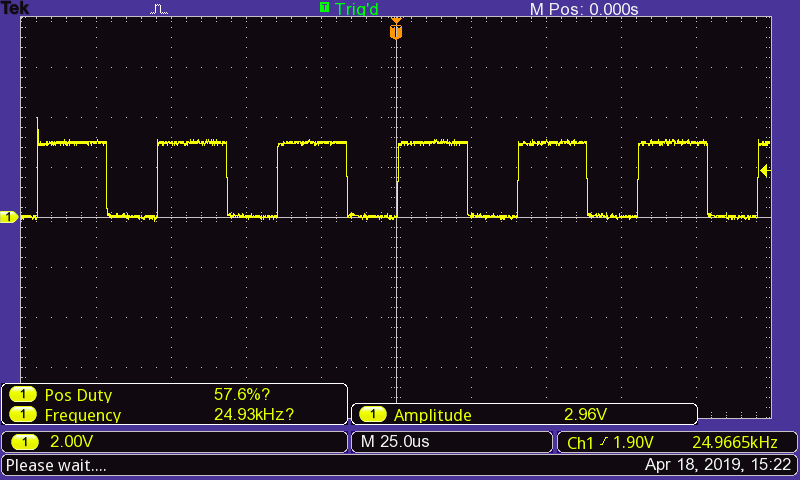
\includegraphics[width=\textwidth]{images/pwm_input_from_pi.png}
  \caption{Shows the input to the MOSFET driver IC (ICL7667 chip) from the Raspberry Pi}
  \label{fig:pwm_input_from_pi}
\end{figure}

We see that the input to the driver is a digital signal with the desired switching frequency of $\approx 25$KHz. The peak voltage is $2.96$V, not enough to turn on the MOSFET. The MOSFET driver is used to step up this voltage to some provided voltage, see the figure that follows for more.

\begin{figure}[H]
  \centering
  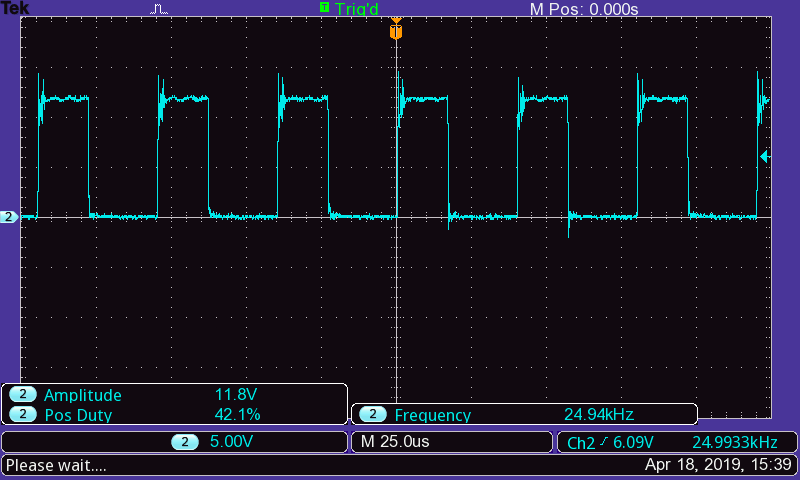
\includegraphics[width=\textwidth]{images/pwm_output_from_chip.png}
  \caption{The PWM output of the ICL7667 chip}
  \label{fig:pwm_output_from_chip}
\end{figure}


This is the voltage fed to the gate terminal of the IRF510 MOSFET (after the
capacitor ridding the signal of voltage spikes). The ICL7667 takes as an input
voltage the $12$V from the supply (even though the datasheet of the IRF510
MOSFET requires a minimum of $5$V across the gate-source terminals to turn on,
the $12$V supply was taken because it is easily available from the input supply
to the circuit). A minimization of the voltage spikes during transition from
the off state to the on state resulted due to the addition of the capacitor.
The voltage spikes and ringing of the voltage can be explained by the unwanted
inductance in the critical loop of the circuit (the critical loop is loop
containing the input supply, inductance $L1$ and the NMOS MOSFET of Figure
\ref{fig:circuit_diagram}). \\

Figure \ref{fig:pwm_output_from_chip} also shows the maximum duty cycle of $\approx 42.5\%$ evident with the maximum load connected, controlled by the feedback system. \\

\begin{figure}[H]
  \centering
  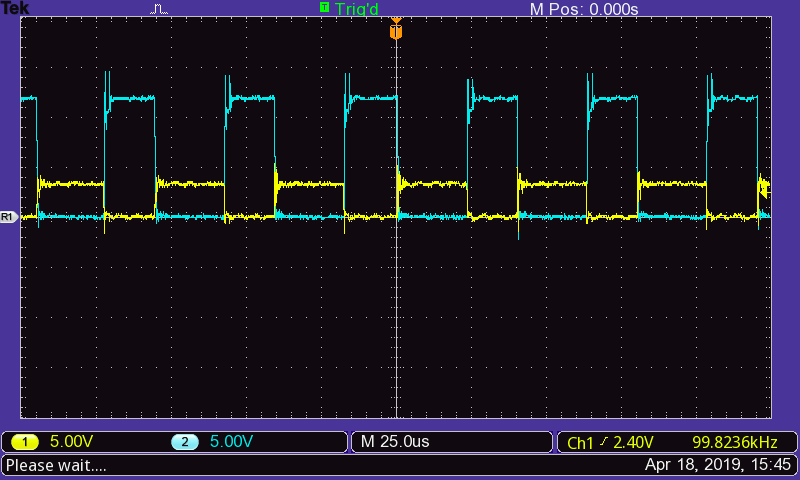
\includegraphics[width=\textwidth]{images/pwm_input_output_comparison.png}
  \caption{A comparison of the input signal from the raspberry pi to the MOSFET driver (the yellow trace) and the output of the MOSFET driver (blue trace)}
  \label{fig:pwm_input_output_comparison}
\end{figure}

Figure \ref{fig:pwm_input_output_comparison} shows the supper-position of the
MOSFET input signal and output signal as already discussed.\\

\begin{figure}[H]
  \centering
  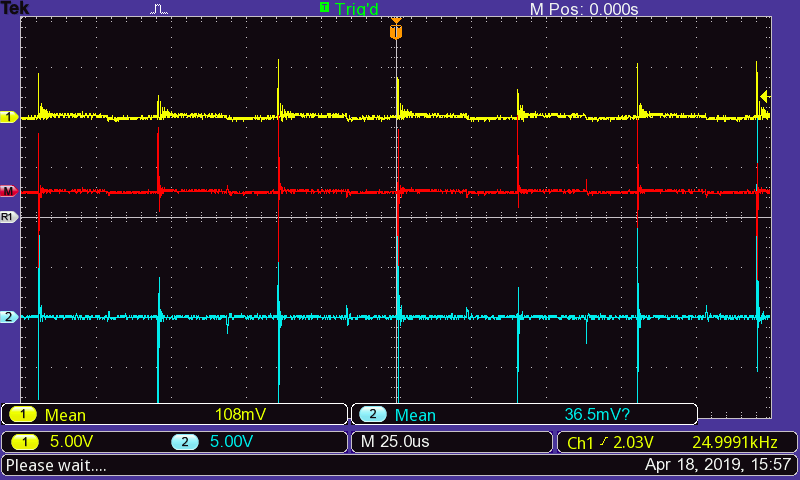
\includegraphics[width=\textwidth]{images/VDS.png}
  \caption{Drain to source voltage of the IRF510 MOSFET, the blue trace shows the voltage across the source of the MOSFET and the yellow trace shows the drain voltage}
  \label{fig:vds}
\end{figure} 

The drain voltage (yellow trace from Figure \ref{fig:vds}) shows ringing, this is not due to inductance alone rather it is explained by the combined effect of inductance (inductance of the MOSFET as well as the inductor) and capacitance (the capacitance is introduced by the MOSFET). We also see that the MOSFET voltage drop during the on mode is $\approx 1$V (the difference between the yellow trace and the blue trace during an on cycle is $1$V).
 
\begin{figure}[H]
  \centering
  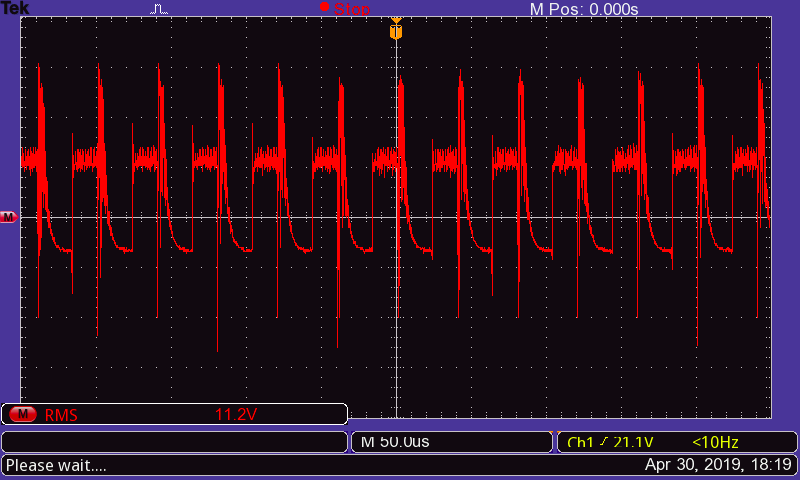
\includegraphics[width=\textwidth]{images/Primary.png}
  \caption{Primary side voltage of the inductor}
  \label{fig:primary}
\end{figure} 

Figure \ref{fig:primary} shows the same oscillations as with the ringing across the drain and the source terminals of the MOSFET (Figure \ref{fig:vds}). Again the oscillation is explained by the capacitance of the MOSFET. The rms voltage lies close to $11$V which is expected, there is a $1$V voltage drop across the MOSFET when it's in the on mode due to the $R_{DS}$ resistance of the MOSFET which was designed for.  


\begin{figure}[H]
  \centering
  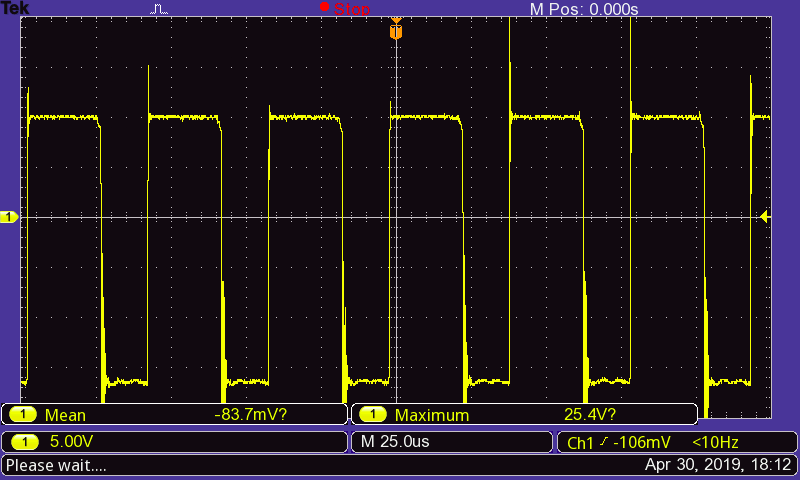
\includegraphics[width=\textwidth]{images/Secondary.png}
  \caption{Secondary voltage of the inductor}
  \label{fig:secondary}
\end{figure} 

The voltage across the secondary as can be seen from Figure \ref{fig:secondary} peaks at $\approx 10V$ during the off time of the MOSFET while the voltage drops to a minimum of approximately $\approx -16$V. From the plot we can see that our inductor design is flawed, we would ideally expect to see $\approx 19$V (see equation \eqref{eq:rho}) during the off time - the difference is explained by the leakage inductance of the inductor. The reverse voltage during the on time of the MOSFET also ideally has to be $-19$V, the difference to the true value can be explained due to copper losses in the windings.  Ringing is again evident on the secondary side again explained by the LC components of the secondary circuit.


\begin{figure}[H]
  \centering
  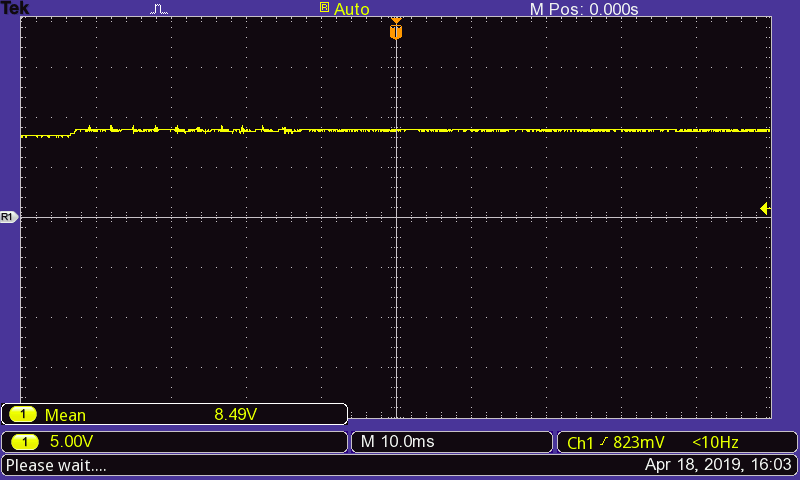
\includegraphics[width=\textwidth]{images/output_from_load.png}
  \caption{The output voltage of the load}
  \label{fig:output_from_load}
\end{figure}. 

Figure \ref{fig:output_from_load} shows the output voltage measure across the $16.5\Omega$ load. The desired voltage of $18$V was not obtained because of the leakage inductance of the core as previously mentioned. The leakage inductance of the core was measured to test our theory. By short circuiting the primary-side and using an LCR meter to find the inductance on the secondary side and performing the same procedure on the secondary-side we found the leakage inductances to be $L_{Pleak} = 0.49mH$ and $L_{Sleak} = 0.18mH$ respectively. Compared to the total inductances of the primary and the secondary of $0.572mH$ and $1.44mH$ respectively, a leakage inductance percentage of $86\%$ and $12.5\%$ respectively, our theory was proved.\\

The core used wasn't gapped by design --- we gapped it ourselves using masking tape. If a gapped core was used, less leakage inductance would have resulted around the air gap and the results would have been closer to the expected value.

\section{Simulations} % (fold)
  \label{sec:simulations}

  \begin{figure}[H]
  \centering
  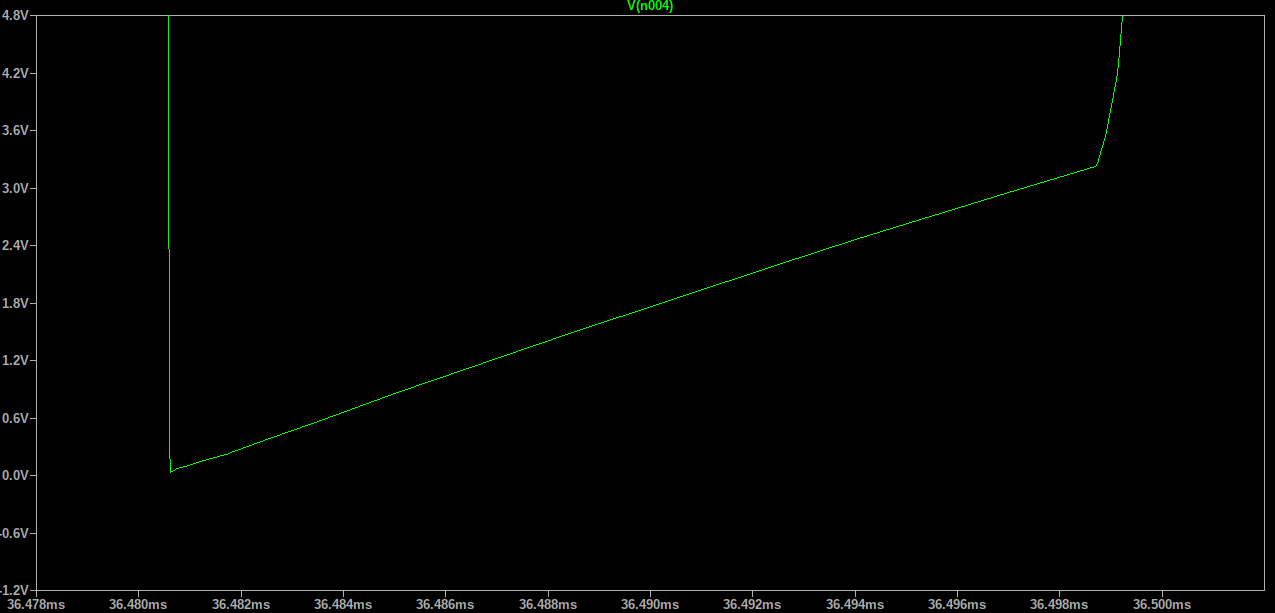
\includegraphics[width=\textwidth]{images/vds_on_sim.png}
  \caption{The simulation of the on voltage of the drain to source of the MOSFET}
  \label{fig:vds_on_sim}
\end{figure} 
Figure \ref{fig:vds_on_sim} shows a voltage drop average of $\approx 1.5$V when the MOSFET conducts, a very similar result was obtained experimentally as shown by Figure \ref{fig:vds}.

\begin{figure}[H]
  \centering
  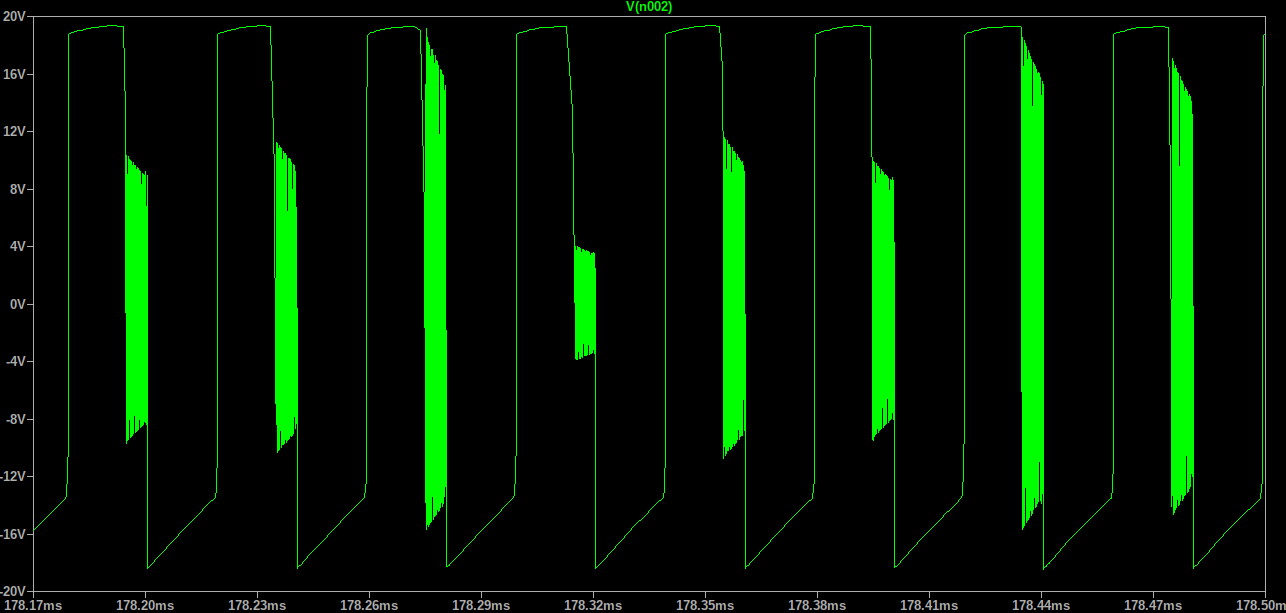
\includegraphics[width=\textwidth]{images/secondary_sim.png}
  \caption{Simulation of the secondary voltage across the coupled inductor}
  \label{fig:secondary_sim}
\end{figure} 

The ringing of the circuit is also portrayed in the simulation however a big difference in the voltage minimum and maximum exists when compared to that of the practical flyback converter (Figure \ref{fig:secondary}). The secondary voltage of the simulation (Figure \ref{fig:secondary_sim}) is close to ideal (as discussed in the results section of this report under the consideration of secondary voltage) as it doesn't incorporate the leakage inductance.

\begin{figure}[H]
  \centering
  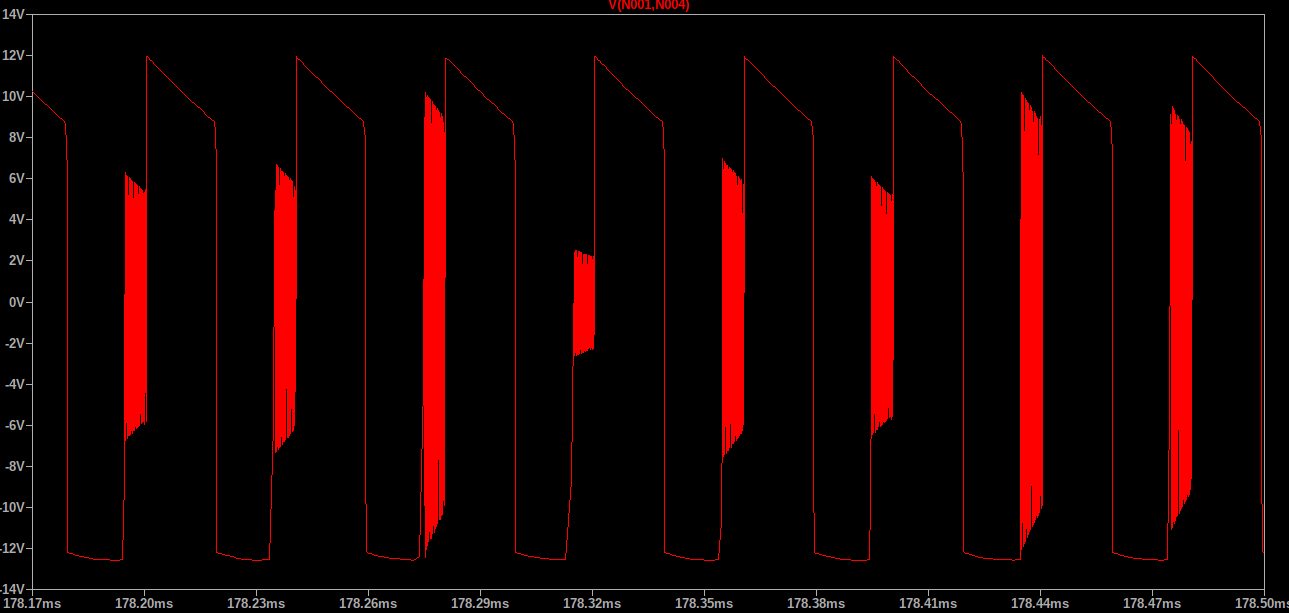
\includegraphics[width=\textwidth]{images/primary_sim.png}
  \caption{Simulation of the primary voltage across the coupled inductor}
  \label{fig:primary_sim}
\end{figure}

No voltage spike exists because the parasitic inductance of the components in the simulation are assumed to be negligibly small, there does exists the oscillations due to the capacitance and the inductance however because the inductance isn't exactly $0$ and capacitance of the MOSFET is also considered in the simulation (the IRF510 MOSFET was given).

\begin{figure}[H]
  \centering
  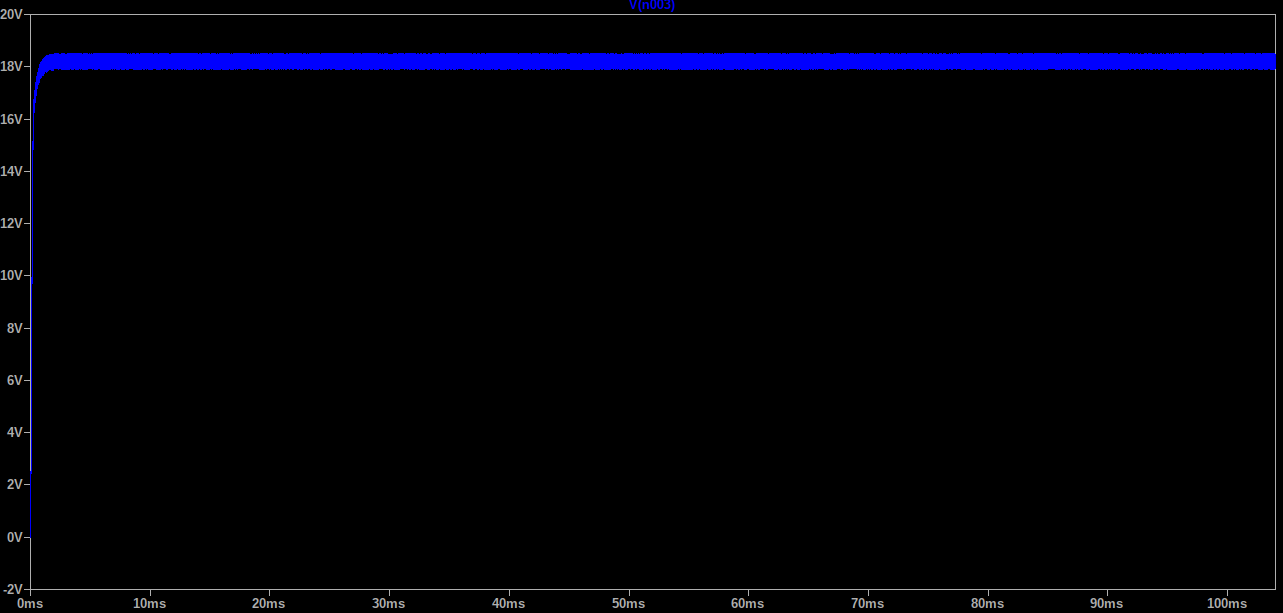
\includegraphics[width=\textwidth]{images/output_1_sim.png}
  \caption{Simulation of the output voltage showing the transients and the final value of the output voltage}
  \label{fig:output_1_sim}
\end{figure} 

Figure \ref{fig:output_1_sim} shows the transients of the system dying out and a steady state voltage of the desired value.

\begin{figure}[H]
  \centering
  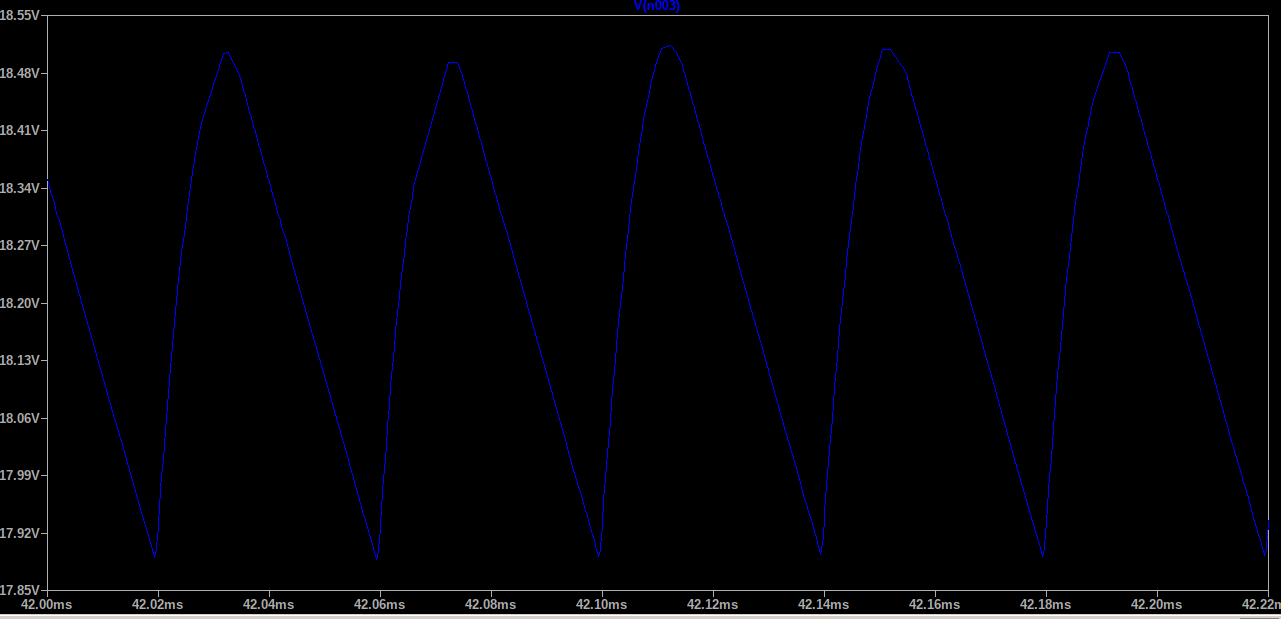
\includegraphics[width=\textwidth]{images/output_2_sim.png}
  \caption{Simulation of the steady state voltage}
  \label{fig:output_2_sim}
\end{figure}

Figure \ref{fig:output_2_sim} illustrates the voltage ripple that exists due to current flowing when the MOSFET is in the off mode and not flowing when the MOSFET conducts. The ripple is within the designed for value of $10\%$. 
  
  % section simulations (end)  

% endsection Results and Discussion

\begin{thebibliography}{0}
	\bibitem{pressman} A. Pressman, K. Billings, T. Morey, \textit{Switching Power Supply Design, Third Edition}, Chapter 4 --- Flyback Converter Topologies
	\bibitem{pwe_conv_applications} N. Mohan, T. M. Undeland, W. P. Robbins, \textit{Power Electronics --- Converters, Applications, and Design, Second Edition}, Chapter 10.4.2 
\end{thebibliography}

\newpage
\begin{appendices}
	\section{Negative Feedback Code}
	\label{sec:feedback_code}
	Below is the code that was implemented for negative feedback control in
	the Raspberry Pi. The code was implemented in the C programming
	language, and compiled using the GCC compiler with the relevant
	compiling flags to the libraries used. Note that the algorithm
	implements a PI type controller. The reasoning for this specific choice
	came from a lecture on PWM control in Power Electronics, where Dr.
	Pentz stated that an integrator constant acts as a low-pass filter,
	avoiding excessive readings from noise, whereas a derivative constant
	acts as a high-pass filter, increasing the noise instead.
	
	Lastly, it's worth noting that this algorithm was able to execute
	successfully without any significant impact on the PWM frequency, due
	to the Raspberry Pi's processing speed, and the use of threads for
	concurrent processing. There is some code that takes user input in the
	main function. This was simply for demonstration purposes, so we could
	easily run the PWM program through the terminal, and safely quit all
	the threads with a single command.\\\\\noindent
	\texttt{\#include <wiringPi.h>} \\\noindent
	\texttt{\#include <stdio.h>} \\\noindent
	\texttt{\#include <stdlib.h>} \\\noindent
	\texttt{\#include <stdint.h>} \\\noindent
	\texttt{\#include <time.h>} \\\noindent
	\texttt{\#include <pthread.h>} \\\noindent
	\texttt{\#include <math.h>} \\\noindent
	\texttt{\#include <stdbool.h>} \\\noindent
	\texttt{\#include <mcp3004.h>} \\\noindent
	\texttt{ \\\noindent}
	\texttt{\#define BASE 100} \\\noindent
	\texttt{\#define SPI\_CHAN 0} \\\noindent
	\texttt{ \\\noindent}
	\texttt{double period = 40;} \\\noindent
	\texttt{const double D\_MAX = 0.425;} \\\noindent
	\texttt{const double D\_MIN = 0.025;} \\\noindent
	\texttt{double duty\_cycle = 0.425;} \\\noindent
	\texttt{int voltage = 0;} \\\noindent
	\texttt{double normalized\_voltage = 0.0;} \\\noindent
	\texttt{double error = 0.0;} \\\noindent
	\texttt{int ref\_voltage = 18;} \\\noindent
	\texttt{const int vref = 5;} \\\noindent
	\texttt{const double r\_factor = 11 * 5.2 / 1024;} \\\noindent
	\texttt{double p = 0.0125;} \\\noindent
	\texttt{double p\_i = 0.003;} \\\noindent
	\texttt{ \\\noindent}
	\texttt{bool running = true;} \\\noindent
	\texttt{ \\\noindent}
	\texttt{void *run\_pwm()} \\\noindent
	\texttt{\{ \\\noindent}
	\texttt{ \\\noindent}
	\texttt{\hspace*{1em}double fixed\_cycle = 0;} \\\noindent
	\texttt{\hspace*{1em}int t\_on = 0;} \\\noindent
	\texttt{\hspace*{1em}int t\_off = 0;} \\\noindent
	\texttt{\hspace*{1em}int x;} \\\noindent
	\texttt{\hspace*{1em}while(running)\{ \\\noindent}
	\texttt{\hspace*{2em}fixed\_cycle = duty\_cycle;} \\\noindent
	\texttt{\hspace*{2em}t\_on = round(period * fixed\_cycle);} \\\noindent
	\texttt{\hspace*{2em}t\_off = round(period * (1 - fixed\_cycle));} \\\noindent
	\texttt{\hspace*{2em}digitalWrite(1, LOW);} \\\noindent
	\texttt{\hspace*{2em}delayMicroseconds(t\_on);} \\\noindent
	\texttt{\hspace*{2em}digitalWrite(1, HIGH);} \\\noindent
	\texttt{\hspace*{2em}delayMicroseconds(t\_off);} \\\noindent
      \texttt{\hspace*{1em}\}} \\\noindent
	\texttt{\hspace*{1em}	} \\\noindent
	\texttt{\hspace*{1em}// Clean up the output pins for safety} \\\noindent
	\texttt{\hspace*{1em}digitalWrite(1, LOW);} \\\noindent
	\texttt{\hspace*{1em}pinMode(1, 0);} \\\noindent
	\texttt{\hspace*{1em}}\\\noindent
        \texttt{ \\\noindent}
        \texttt{void *controller()} \\\noindent
        \texttt{\{ \\\noindent}
	\texttt{\hspace*{1em}const int size\_max = 10;} \\\noindent
	\texttt{\hspace*{1em}double i\_values[10] = \{\};} \\\noindent
	\texttt{\hspace*{1em}size = 0;} \\\noindent
	\texttt{\hspace*{1em}double sum = 0;} \\\noindent
	\texttt{\hspace*{1em}while(running)} \\\noindent
	\texttt{\hspace*{2em}\{ \\\noindent}
	\texttt{\hspace*{2em}// run until cancel} \\\noindent
	\texttt{\hspace*{2em}// get measurements} \\\noindent
	\texttt{\hspace*{2em}voltage = analogRead(BASE);} \\\noindent
	\texttt{\hspace*{2em}normalized\_voltage = voltage * r\_factor;} \\\noindent
	\texttt{\hspace*{2em}error = ref\_voltage - normalized\_voltage;} \\\noindent
	\texttt{\hspace*{2em}\\\noindent}
	\texttt{\hspace*{2em}// Add error value to integrator} \\\noindent
	\texttt{\hspace*{2em}if(size < size\_max) \{ \\\noindent}
	\texttt{\hspace*{3em}size++;} \\\noindent
	\texttt{\hspace*{3em}i\_values[size - 1] = error;} \\\noindent
	\texttt{\hspace*{2em}\}} \\\noindent
	\texttt{\hspace*{2em}else \{ \\\noindent}
	\texttt{\hspace*{3em}// shift old values} \\\noindent
	\texttt{\hspace*{3em}int i;} \\\noindent
	\texttt{\hspace*{3em}for(i = 0; i < size\_max - 1; i++)} \\\noindent
	\texttt{\hspace*{3em}i\_values[i] = i\_values[i + 1];} \\\noindent
	\texttt{\hspace*{3em}i\_values[size\_max - 1] = error;} \\\noindent
	\texttt{\hspace*{2em}\}} \\\noindent
	\texttt{ \\\noindent}
	\texttt{\hspace*{2em}// sum values for integrator} \\\noindent
	\texttt{\hspace*{2em}int i;} \\\noindent
	\texttt{\hspace*{2em}sum = 0;} \\\noindent
	\texttt{\hspace*{2em}for(i = 0; i < size; i++)} \\\noindent
	\texttt{\hspace*{2em}sum += i\_values[i];} \\\noindent
	\texttt{\hspace*{2em}\\\noindent}
	\texttt{\hspace*{2em}// adjust duty cycle accordingly} \\\noindent
	\texttt{\hspace*{2em}duty\_cycle += p * error + p\_i * sum;} \\\noindent
	\texttt{ \\\noindent}
	\texttt{\hspace*{2em}if(duty\_cycle > D\_MAX)} \\\noindent
	\texttt{\hspace*{3em}duty\_cycle = D\_MAX;} \\\noindent
	\texttt{ \\\noindent}
	\texttt{\hspace*{2em}if(duty\_cycle < D\_MIN)} \\\noindent
	\texttt{\hspace*{3em}duty\_cycle = D\_MIN;} \\\noindent
	\texttt{ \\\noindent}
	\texttt{\hspace*{2em}delayMicroseconds(500);} \\\noindent
	\texttt{\hspace*{1em}\}}\\\noindent
        \texttt{\}} \\\noindent
        \texttt{ \\\noindent}

	\texttt{main(void) \{ \\\noindent}
	\texttt{\hspace*{1em}// setup physical} \\\noindent
	\texttt{\hspace*{1em}wiringPiSetup();} \\\noindent
	\texttt{\hspace*{1em}mcp3004Setup(BASE, SPI\_CHAN);} \\\noindent
	\texttt{\hspace*{1em}pinMode(1, OUTPUT); } \\\noindent
	\texttt{\hspace*{1em}\\\noindent}
	\texttt{\hspace*{1em}pthread\_t thread\_1;} \\\noindent
	\texttt{\hspace*{1em}pthread\_t thread\_2;} \\\noindent
	\texttt{\hspace*{1em}pthread\_create(\&thread\_1, NULL, run\_pwm, NULL);} \\\noindent
	\texttt{\hspace*{1em}pthread\_create(\&thread\_2, NULL, controller, NULL);} \\\noindent
	\texttt{\hspace*{1em}\\\noindent}
	\texttt{\hspace*{1em}char* line = NULL;} \\\noindent
	\texttt{\hspace*{1em}size\_t len = 0;} \\\noindent
	\texttt{\hspace*{1em}ssize\_t read = 0;} \\\noindent
	\texttt{\hspace*{1em}\\\noindent}
	\texttt{\hspace*{1em}while(running)} \\\noindent
	\texttt{\hspace*{2em}\{ \\\noindent}
	\texttt{\hspace*{2em}while (read != -1) \{ \\\noindent}
	\texttt{\hspace*{3em}puts("Enter q to quit");} \\\noindent
	\texttt{\hspace*{3em}read = getline(\&line, \&len, stdin);} \\\noindent
	\texttt{\hspace*{3em}puts("");} \\\noindent
	\texttt{\hspace*{3em}if (!strcmp(line, "q")) \{ \\\noindent}
	\texttt{\hspace*{4em}running = false;} \\\noindent
	\texttt{\hspace*{4em}break;} \\\noindent
	\texttt{\hspace*{3em}\}} \\\noindent
	\texttt{\hspace*{2em}\}} \\\noindent
	\texttt{\hspace*{1em}\}} \\\noindent
	\texttt{\hspace*{1em}\\\noindent}
	\texttt{\hspace*{1em}free(line);} \\\noindent
	\texttt{\hspace*{1em}pthread\_join(thread\_1, NULL);} \\\noindent
	\texttt{\hspace*{1em}pthread\_join(thread\_2, NULL);} \\\noindent
	\texttt{\hspace*{1em}\\\noindent}
	\texttt{\hspace*{1em}return 0;} \\\noindent
        \texttt{\}} \\\noindent

\end{appendices}

\end{document}
